\documentclass[twoside]{book}

% Packages required by doxygen
\usepackage{fixltx2e}
\usepackage{calc}
\usepackage{doxygen}
\usepackage[export]{adjustbox} % also loads graphicx
\usepackage{graphicx}
\usepackage[utf8]{inputenc}
\usepackage{makeidx}
\usepackage{multicol}
\usepackage{multirow}
\PassOptionsToPackage{warn}{textcomp}
\usepackage{textcomp}
\usepackage[nointegrals]{wasysym}
\usepackage[table]{xcolor}

% NLS support packages
\usepackage[spanish]{babel}
% Font selection
\usepackage[T1]{fontenc}
\usepackage[scaled=.90]{helvet}
\usepackage{courier}
\usepackage{amssymb}
\usepackage{sectsty}
\renewcommand{\familydefault}{\sfdefault}
\allsectionsfont{%
  \fontseries{bc}\selectfont%
  \color{darkgray}%
}
\renewcommand{\DoxyLabelFont}{%
  \fontseries{bc}\selectfont%
  \color{darkgray}%
}
\newcommand{\+}{\discretionary{\mbox{\scriptsize$\hookleftarrow$}}{}{}}

% Page & text layout
\usepackage{geometry}
\geometry{%
  a4paper,%
  top=2.5cm,%
  bottom=2.5cm,%
  left=2.5cm,%
  right=2.5cm%
}
\tolerance=750
\hfuzz=15pt
\hbadness=750
\setlength{\emergencystretch}{15pt}
\setlength{\parindent}{0cm}
\setlength{\parskip}{3ex plus 2ex minus 2ex}
\makeatletter
\renewcommand{\paragraph}{%
  \@startsection{paragraph}{4}{0ex}{-1.0ex}{1.0ex}{%
    \normalfont\normalsize\bfseries\SS@parafont%
  }%
}
\renewcommand{\subparagraph}{%
  \@startsection{subparagraph}{5}{0ex}{-1.0ex}{1.0ex}{%
    \normalfont\normalsize\bfseries\SS@subparafont%
  }%
}
\makeatother

% Headers & footers
\usepackage{fancyhdr}
\pagestyle{fancyplain}
\fancyhead[LE]{\fancyplain{}{\bfseries\thepage}}
\fancyhead[CE]{\fancyplain{}{}}
\fancyhead[RE]{\fancyplain{}{\bfseries\leftmark}}
\fancyhead[LO]{\fancyplain{}{\bfseries\rightmark}}
\fancyhead[CO]{\fancyplain{}{}}
\fancyhead[RO]{\fancyplain{}{\bfseries\thepage}}
\fancyfoot[LE]{\fancyplain{}{}}
\fancyfoot[CE]{\fancyplain{}{}}
\fancyfoot[RE]{\fancyplain{}{\bfseries\scriptsize Generado por Doxygen }}
\fancyfoot[LO]{\fancyplain{}{\bfseries\scriptsize Generado por Doxygen }}
\fancyfoot[CO]{\fancyplain{}{}}
\fancyfoot[RO]{\fancyplain{}{}}
\renewcommand{\footrulewidth}{0.4pt}
\renewcommand{\chaptermark}[1]{%
  \markboth{#1}{}%
}
\renewcommand{\sectionmark}[1]{%
  \markright{\thesection\ #1}%
}

% Indices & bibliography
\usepackage{natbib}
\usepackage[titles]{tocloft}
\setcounter{tocdepth}{3}
\setcounter{secnumdepth}{5}
\makeindex

% Hyperlinks (required, but should be loaded last)
\usepackage{ifpdf}
\ifpdf
  \usepackage[pdftex,pagebackref=true]{hyperref}
\else
  \usepackage[ps2pdf,pagebackref=true]{hyperref}
\fi
\hypersetup{%
  colorlinks=true,%
  linkcolor=blue,%
  citecolor=blue,%
  unicode%
}

% Custom commands
\newcommand{\clearemptydoublepage}{%
  \newpage{\pagestyle{empty}\cleardoublepage}%
}

\usepackage{caption}
\captionsetup{labelsep=space,justification=centering,font={bf},singlelinecheck=off,skip=4pt,position=top}

%===== C O N T E N T S =====

\begin{document}

% Titlepage & ToC
\hypersetup{pageanchor=false,
             bookmarksnumbered=true,
             pdfencoding=unicode
            }
\pagenumbering{alph}
\begin{titlepage}
\vspace*{7cm}
\begin{center}%
{\Large Air\+Combat \\[1ex]\large 1.\+0 }\\
\vspace*{1cm}
{\large Generado por Doxygen 1.8.12}\\
\end{center}
\end{titlepage}
\clearemptydoublepage
\pagenumbering{roman}
\tableofcontents
\clearemptydoublepage
\pagenumbering{arabic}
\hypersetup{pageanchor=true}

%--- Begin generated contents ---
\chapter{Indice jerárquico}
\section{Jerarquía de la clase}
Esta lista de herencias esta ordenada aproximadamente por orden alfabético\+:\begin{DoxyCompactList}
\item \contentsline{section}{Enemy}{\pageref{class_enemy}}{}
\begin{DoxyCompactList}
\item \contentsline{section}{Basic\+Enemy}{\pageref{class_basic_enemy}}{}
\item \contentsline{section}{Boss\+Enemy}{\pageref{class_boss_enemy}}{}
\end{DoxyCompactList}
\item Q\+Graphics\+Pixmap\+Item\begin{DoxyCompactList}
\item \contentsline{section}{Back\+Ground}{\pageref{class_back_ground}}{}
\item \contentsline{section}{Basic\+Enemy}{\pageref{class_basic_enemy}}{}
\item \contentsline{section}{Boss\+Enemy}{\pageref{class_boss_enemy}}{}
\item \contentsline{section}{Bullet}{\pageref{class_bullet}}{}
\item \contentsline{section}{Player}{\pageref{class_player}}{}
\end{DoxyCompactList}
\item Q\+Graphics\+Rect\+Item\begin{DoxyCompactList}
\item \contentsline{section}{Button}{\pageref{class_button}}{}
\end{DoxyCompactList}
\item Q\+Graphics\+Text\+Item\begin{DoxyCompactList}
\item \contentsline{section}{Enemy\+Controller}{\pageref{class_enemy_controller}}{}
\item \contentsline{section}{Healht}{\pageref{class_healht}}{}
\item \contentsline{section}{Score}{\pageref{class_score}}{}
\end{DoxyCompactList}
\item Q\+Graphics\+View\begin{DoxyCompactList}
\item \contentsline{section}{Game}{\pageref{class_game}}{}
\end{DoxyCompactList}
\item Q\+Object\begin{DoxyCompactList}
\item \contentsline{section}{Basic\+Enemy}{\pageref{class_basic_enemy}}{}
\item \contentsline{section}{Boss\+Enemy}{\pageref{class_boss_enemy}}{}
\item \contentsline{section}{Bullet}{\pageref{class_bullet}}{}
\item \contentsline{section}{Button}{\pageref{class_button}}{}
\item \contentsline{section}{Player}{\pageref{class_player}}{}
\end{DoxyCompactList}
\end{DoxyCompactList}

\chapter{Índice de clases}
\section{Lista de clases}
Lista de las clases, estructuras, uniones e interfaces con una breve descripción\+:\begin{DoxyCompactList}
\item\contentsline{section}{\hyperlink{class_back_ground}{Back\+Ground} }{\pageref{class_back_ground}}{}
\item\contentsline{section}{\hyperlink{class_basic_enemy}{Basic\+Enemy} }{\pageref{class_basic_enemy}}{}
\item\contentsline{section}{\hyperlink{class_boss_enemy}{Boss\+Enemy} }{\pageref{class_boss_enemy}}{}
\item\contentsline{section}{\hyperlink{class_bullet}{Bullet} }{\pageref{class_bullet}}{}
\item\contentsline{section}{\hyperlink{class_button}{Button} }{\pageref{class_button}}{}
\item\contentsline{section}{\hyperlink{class_enemy}{Enemy} }{\pageref{class_enemy}}{}
\item\contentsline{section}{\hyperlink{class_enemy_controller}{Enemy\+Controller} }{\pageref{class_enemy_controller}}{}
\item\contentsline{section}{\hyperlink{class_game}{Game} }{\pageref{class_game}}{}
\item\contentsline{section}{\hyperlink{class_healht}{Healht} }{\pageref{class_healht}}{}
\item\contentsline{section}{\hyperlink{class_player}{Player} }{\pageref{class_player}}{}
\item\contentsline{section}{\hyperlink{class_score}{Score} }{\pageref{class_score}}{}
\end{DoxyCompactList}

\chapter{Indice de archivos}
\section{Lista de archivos}
Lista de todos los archivos con descripciones breves\+:\begin{DoxyCompactList}
\item\contentsline{section}{\hyperlink{background_8cpp}{background.\+cpp} }{\pageref{background_8cpp}}{}
\item\contentsline{section}{\hyperlink{background_8h}{background.\+h} \\*This class is for place the image background at star of the game }{\pageref{background_8h}}{}
\item\contentsline{section}{\hyperlink{basicenemy_8cpp}{basicenemy.\+cpp} }{\pageref{basicenemy_8cpp}}{}
\item\contentsline{section}{\hyperlink{basicenemy_8h}{basicenemy.\+h} \\*This class is to representation of basic enemy if you killed basic enemy you score increase if you score is more of 10 your live increase in 50 }{\pageref{basicenemy_8h}}{}
\item\contentsline{section}{\hyperlink{bossenemy_8cpp}{bossenemy.\+cpp} }{\pageref{bossenemy_8cpp}}{}
\item\contentsline{section}{\hyperlink{bossenemy_8h}{bossenemy.\+h} \\*This class is toa representation a boss enemy if you killed a boss enemy you win the game }{\pageref{bossenemy_8h}}{}
\item\contentsline{section}{\hyperlink{bullet_8cpp}{bullet.\+cpp} }{\pageref{bullet_8cpp}}{}
\item\contentsline{section}{\hyperlink{bullet_8h}{bullet.\+h} }{\pageref{bullet_8h}}{}
\item\contentsline{section}{\hyperlink{button_8cpp}{button.\+cpp} }{\pageref{button_8cpp}}{}
\item\contentsline{section}{\hyperlink{button_8h}{button.\+h} \\*This class is for create button for start or quit of the game }{\pageref{button_8h}}{}
\item\contentsline{section}{\hyperlink{enemy_8cpp}{enemy.\+cpp} }{\pageref{enemy_8cpp}}{}
\item\contentsline{section}{\hyperlink{enemy_8h}{enemy.\+h} }{\pageref{enemy_8h}}{}
\item\contentsline{section}{\hyperlink{enemycontroller_8cpp}{enemycontroller.\+cpp} }{\pageref{enemycontroller_8cpp}}{}
\item\contentsline{section}{\hyperlink{enemycontroller_8h}{enemycontroller.\+h} \\*This class is for controller enemy for exmaple to control your live or number enemies }{\pageref{enemycontroller_8h}}{}
\item\contentsline{section}{\hyperlink{game_8cpp}{game.\+cpp} }{\pageref{game_8cpp}}{}
\item\contentsline{section}{\hyperlink{game_8h}{game.\+h} }{\pageref{game_8h}}{}
\item\contentsline{section}{\hyperlink{healht_8cpp}{healht.\+cpp} }{\pageref{healht_8cpp}}{}
\item\contentsline{section}{\hyperlink{healht_8h}{healht.\+h} }{\pageref{healht_8h}}{}
\item\contentsline{section}{\hyperlink{main_8cpp}{main.\+cpp} }{\pageref{main_8cpp}}{}
\item\contentsline{section}{\hyperlink{player_8cpp}{player.\+cpp} }{\pageref{player_8cpp}}{}
\item\contentsline{section}{\hyperlink{player_8h}{player.\+h} }{\pageref{player_8h}}{}
\item\contentsline{section}{\hyperlink{score_8cpp}{score.\+cpp} }{\pageref{score_8cpp}}{}
\item\contentsline{section}{\hyperlink{score_8h}{score.\+h} }{\pageref{score_8h}}{}
\end{DoxyCompactList}

\chapter{Documentación de las clases}
\hypertarget{class_back_ground}{}\section{Referencia de la Clase Back\+Ground}
\label{class_back_ground}\index{Back\+Ground@{Back\+Ground}}


{\ttfamily \#include $<$background.\+h$>$}

Diagrama de herencias de Back\+Ground\begin{figure}[H]
\begin{center}
\leavevmode
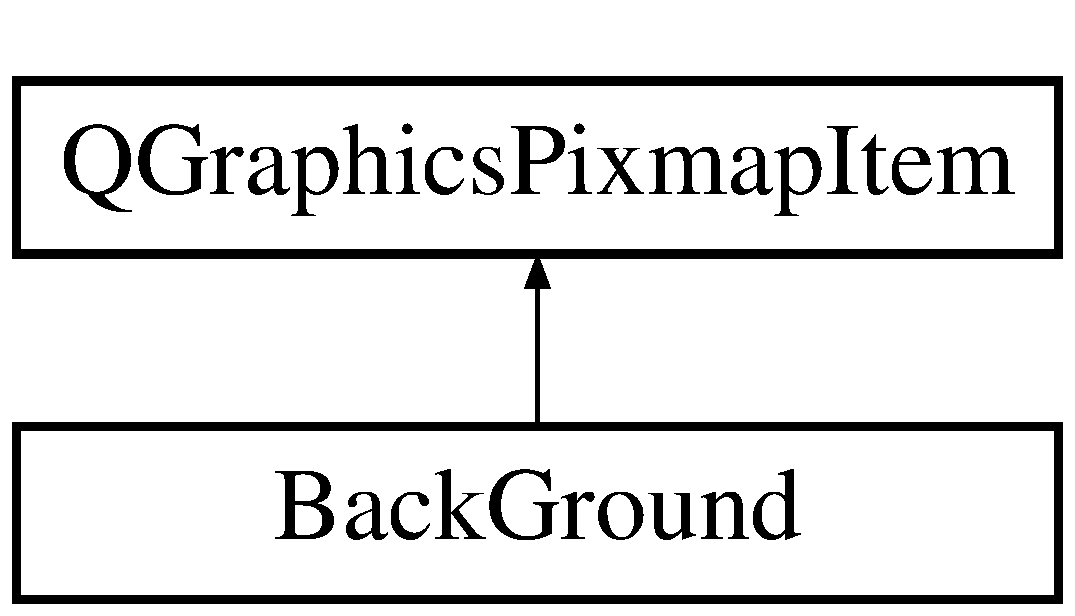
\includegraphics[height=2.000000cm]{class_back_ground}
\end{center}
\end{figure}
\subsection*{Métodos públicos}
\begin{DoxyCompactItemize}
\item 
\hyperlink{class_back_ground_a6a3fe7aa2ec8d57d372d336cd2d64337}{Back\+Ground} ()
\end{DoxyCompactItemize}


\subsection{Documentación del constructor y destructor}
\hypertarget{class_back_ground_a6a3fe7aa2ec8d57d372d336cd2d64337}{}\label{class_back_ground_a6a3fe7aa2ec8d57d372d336cd2d64337} 
\index{Back\+Ground@{Back\+Ground}!Back\+Ground@{Back\+Ground}}
\index{Back\+Ground@{Back\+Ground}!Back\+Ground@{Back\+Ground}}
\subsubsection{\texorpdfstring{Back\+Ground()}{BackGround()}}
{\footnotesize\ttfamily Back\+Ground\+::\+Back\+Ground (\begin{DoxyParamCaption}{ }\end{DoxyParamCaption})}



La documentación para esta clase fue generada a partir de los siguientes ficheros\+:\begin{DoxyCompactItemize}
\item 
\hyperlink{background_8h}{background.\+h}\item 
\hyperlink{background_8cpp}{background.\+cpp}\end{DoxyCompactItemize}

\hypertarget{class_basic_enemy}{}\section{Referencia de la Clase Basic\+Enemy}
\label{class_basic_enemy}\index{Basic\+Enemy@{Basic\+Enemy}}


{\ttfamily \#include $<$basicenemy.\+h$>$}

Diagrama de herencias de Basic\+Enemy\begin{figure}[H]
\begin{center}
\leavevmode
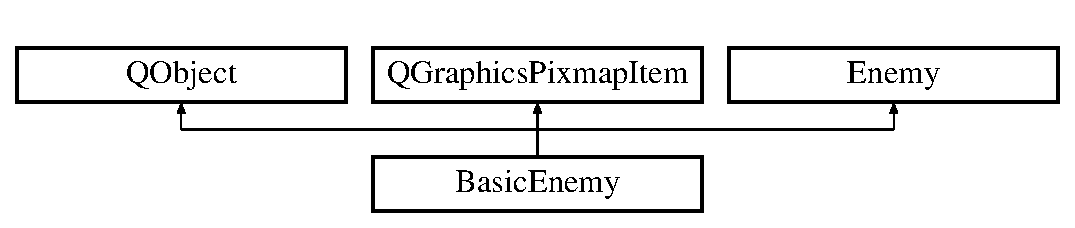
\includegraphics[height=2.000000cm]{class_basic_enemy}
\end{center}
\end{figure}
\subsection*{Slots públicos}
\begin{DoxyCompactItemize}
\item 
void \hyperlink{class_basic_enemy_ad491ec5aa0aee2b51399181f5e8259db}{move} ()
\end{DoxyCompactItemize}
\subsection*{Métodos públicos}
\begin{DoxyCompactItemize}
\item 
\hyperlink{class_basic_enemy_a1e97e4012172888af93dc1286dc4ade0}{Basic\+Enemy} ()
\end{DoxyCompactItemize}


\subsection{Documentación del constructor y destructor}
\hypertarget{class_basic_enemy_a1e97e4012172888af93dc1286dc4ade0}{}\label{class_basic_enemy_a1e97e4012172888af93dc1286dc4ade0} 
\index{Basic\+Enemy@{Basic\+Enemy}!Basic\+Enemy@{Basic\+Enemy}}
\index{Basic\+Enemy@{Basic\+Enemy}!Basic\+Enemy@{Basic\+Enemy}}
\subsubsection{\texorpdfstring{Basic\+Enemy()}{BasicEnemy()}}
{\footnotesize\ttfamily Basic\+Enemy\+::\+Basic\+Enemy (\begin{DoxyParamCaption}{ }\end{DoxyParamCaption})}



\subsection{Documentación de las funciones miembro}
\hypertarget{class_basic_enemy_ad491ec5aa0aee2b51399181f5e8259db}{}\label{class_basic_enemy_ad491ec5aa0aee2b51399181f5e8259db} 
\index{Basic\+Enemy@{Basic\+Enemy}!move@{move}}
\index{move@{move}!Basic\+Enemy@{Basic\+Enemy}}
\subsubsection{\texorpdfstring{move}{move}}
{\footnotesize\ttfamily void Basic\+Enemy\+::move (\begin{DoxyParamCaption}{ }\end{DoxyParamCaption})\hspace{0.3cm}{\ttfamily [slot]}}



La documentación para esta clase fue generada a partir de los siguientes ficheros\+:\begin{DoxyCompactItemize}
\item 
\hyperlink{basicenemy_8h}{basicenemy.\+h}\item 
\hyperlink{basicenemy_8cpp}{basicenemy.\+cpp}\end{DoxyCompactItemize}

\hypertarget{class_boss_enemy}{}\section{Referencia de la Clase Boss\+Enemy}
\label{class_boss_enemy}\index{Boss\+Enemy@{Boss\+Enemy}}


{\ttfamily \#include $<$bossenemy.\+h$>$}

Diagrama de herencias de Boss\+Enemy\begin{figure}[H]
\begin{center}
\leavevmode
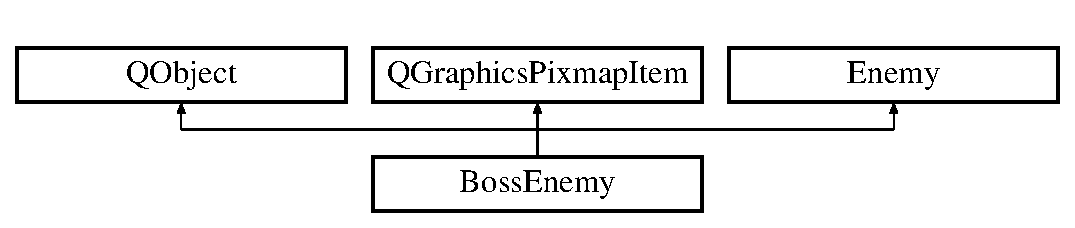
\includegraphics[height=2.000000cm]{class_boss_enemy}
\end{center}
\end{figure}
\subsection*{Slots públicos}
\begin{DoxyCompactItemize}
\item 
void \hyperlink{class_boss_enemy_a25a9f61fe3b4770b72a9dccb7685f2e9}{move} ()
\end{DoxyCompactItemize}
\subsection*{Métodos públicos}
\begin{DoxyCompactItemize}
\item 
\hyperlink{class_boss_enemy_a9240daf56362aa847067d5bad23c7a36}{Boss\+Enemy} ()
\end{DoxyCompactItemize}


\subsection{Documentación del constructor y destructor}
\hypertarget{class_boss_enemy_a9240daf56362aa847067d5bad23c7a36}{}\label{class_boss_enemy_a9240daf56362aa847067d5bad23c7a36} 
\index{Boss\+Enemy@{Boss\+Enemy}!Boss\+Enemy@{Boss\+Enemy}}
\index{Boss\+Enemy@{Boss\+Enemy}!Boss\+Enemy@{Boss\+Enemy}}
\subsubsection{\texorpdfstring{Boss\+Enemy()}{BossEnemy()}}
{\footnotesize\ttfamily Boss\+Enemy\+::\+Boss\+Enemy (\begin{DoxyParamCaption}{ }\end{DoxyParamCaption})}



\subsection{Documentación de las funciones miembro}
\hypertarget{class_boss_enemy_a25a9f61fe3b4770b72a9dccb7685f2e9}{}\label{class_boss_enemy_a25a9f61fe3b4770b72a9dccb7685f2e9} 
\index{Boss\+Enemy@{Boss\+Enemy}!move@{move}}
\index{move@{move}!Boss\+Enemy@{Boss\+Enemy}}
\subsubsection{\texorpdfstring{move}{move}}
{\footnotesize\ttfamily void Boss\+Enemy\+::move (\begin{DoxyParamCaption}{ }\end{DoxyParamCaption})\hspace{0.3cm}{\ttfamily [slot]}}



La documentación para esta clase fue generada a partir de los siguientes ficheros\+:\begin{DoxyCompactItemize}
\item 
\hyperlink{bossenemy_8h}{bossenemy.\+h}\item 
\hyperlink{bossenemy_8cpp}{bossenemy.\+cpp}\end{DoxyCompactItemize}

\hypertarget{class_bullet}{}\section{Referencia de la Clase Bullet}
\label{class_bullet}\index{Bullet@{Bullet}}


{\ttfamily \#include $<$bullet.\+h$>$}

Diagrama de herencias de Bullet\begin{figure}[H]
\begin{center}
\leavevmode
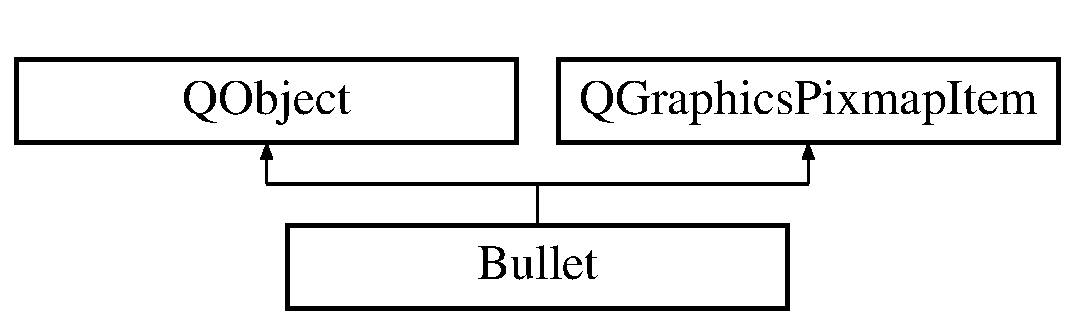
\includegraphics[height=2.000000cm]{class_bullet}
\end{center}
\end{figure}
\subsection*{Slots públicos}
\begin{DoxyCompactItemize}
\item 
void \hyperlink{class_bullet_a6140db968c42c05e829e142f74f20b16}{move} ()
\end{DoxyCompactItemize}
\subsection*{Métodos públicos}
\begin{DoxyCompactItemize}
\item 
\hyperlink{class_bullet_ab0bc0aa71829a6ccd0d488bb61eee065}{Bullet} (int)
\end{DoxyCompactItemize}


\subsection{Documentación del constructor y destructor}
\hypertarget{class_bullet_ab0bc0aa71829a6ccd0d488bb61eee065}{}\label{class_bullet_ab0bc0aa71829a6ccd0d488bb61eee065} 
\index{Bullet@{Bullet}!Bullet@{Bullet}}
\index{Bullet@{Bullet}!Bullet@{Bullet}}
\subsubsection{\texorpdfstring{Bullet()}{Bullet()}}
{\footnotesize\ttfamily Bullet\+::\+Bullet (\begin{DoxyParamCaption}\item[{int}]{speed }\end{DoxyParamCaption})}



\subsection{Documentación de las funciones miembro}
\hypertarget{class_bullet_a6140db968c42c05e829e142f74f20b16}{}\label{class_bullet_a6140db968c42c05e829e142f74f20b16} 
\index{Bullet@{Bullet}!move@{move}}
\index{move@{move}!Bullet@{Bullet}}
\subsubsection{\texorpdfstring{move}{move}}
{\footnotesize\ttfamily void Bullet\+::move (\begin{DoxyParamCaption}{ }\end{DoxyParamCaption})\hspace{0.3cm}{\ttfamily [slot]}}



La documentación para esta clase fue generada a partir de los siguientes ficheros\+:\begin{DoxyCompactItemize}
\item 
\hyperlink{bullet_8h}{bullet.\+h}\item 
\hyperlink{bullet_8cpp}{bullet.\+cpp}\end{DoxyCompactItemize}

\hypertarget{class_button}{}\section{Referencia de la Clase Button}
\label{class_button}\index{Button@{Button}}


{\ttfamily \#include $<$button.\+h$>$}

Diagrama de herencias de Button\begin{figure}[H]
\begin{center}
\leavevmode
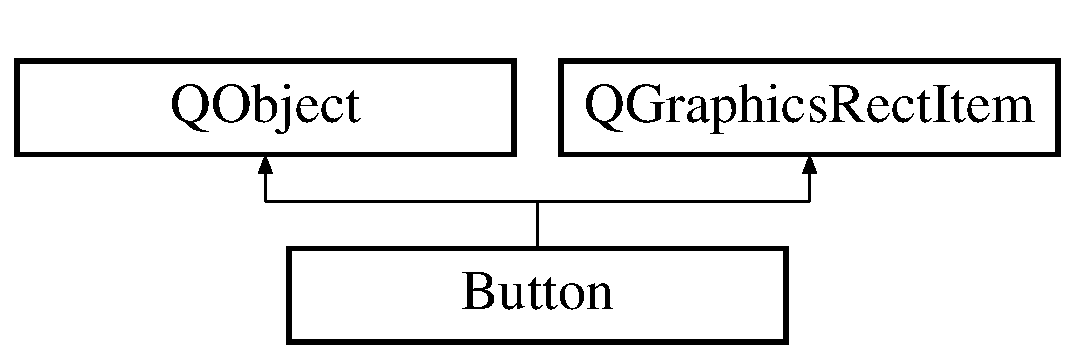
\includegraphics[height=2.000000cm]{class_button}
\end{center}
\end{figure}
\subsection*{Señales}
\begin{DoxyCompactItemize}
\item 
void \hyperlink{class_button_a9e7ab4152cb1e7e3beb7f2842f32670c}{clicked} ()
\end{DoxyCompactItemize}
\subsection*{Métodos públicos}
\begin{DoxyCompactItemize}
\item 
\hyperlink{class_button_a69976e5c00874a3807b642f249c1c776}{Button} (Q\+String name, Q\+Graphics\+Item $\ast$parent=N\+U\+LL)
\item 
void \hyperlink{class_button_a17d8eb0c904605b223bbc00c75655315}{mouse\+Press\+Event} (Q\+Graphics\+Scene\+Mouse\+Event $\ast$event)
\item 
void \hyperlink{class_button_a633a9684818bc5d300a622a00064f09c}{hover\+Enter\+Event} (Q\+Graphics\+Scene\+Hover\+Event $\ast$event)
\item 
void \hyperlink{class_button_a1689a97690d9469ce8350d24db0d7485}{hover\+Leave\+Event} (Q\+Graphics\+Scene\+Hover\+Event $\ast$event)
\end{DoxyCompactItemize}


\subsection{Documentación del constructor y destructor}
\hypertarget{class_button_a69976e5c00874a3807b642f249c1c776}{}\label{class_button_a69976e5c00874a3807b642f249c1c776} 
\index{Button@{Button}!Button@{Button}}
\index{Button@{Button}!Button@{Button}}
\subsubsection{\texorpdfstring{Button()}{Button()}}
{\footnotesize\ttfamily Button\+::\+Button (\begin{DoxyParamCaption}\item[{Q\+String}]{name,  }\item[{Q\+Graphics\+Item $\ast$}]{parent = {\ttfamily NULL} }\end{DoxyParamCaption})}



\subsection{Documentación de las funciones miembro}
\hypertarget{class_button_a9e7ab4152cb1e7e3beb7f2842f32670c}{}\label{class_button_a9e7ab4152cb1e7e3beb7f2842f32670c} 
\index{Button@{Button}!clicked@{clicked}}
\index{clicked@{clicked}!Button@{Button}}
\subsubsection{\texorpdfstring{clicked}{clicked}}
{\footnotesize\ttfamily void Button\+::clicked (\begin{DoxyParamCaption}{ }\end{DoxyParamCaption})\hspace{0.3cm}{\ttfamily [signal]}}

\hypertarget{class_button_a633a9684818bc5d300a622a00064f09c}{}\label{class_button_a633a9684818bc5d300a622a00064f09c} 
\index{Button@{Button}!hover\+Enter\+Event@{hover\+Enter\+Event}}
\index{hover\+Enter\+Event@{hover\+Enter\+Event}!Button@{Button}}
\subsubsection{\texorpdfstring{hover\+Enter\+Event()}{hoverEnterEvent()}}
{\footnotesize\ttfamily void Button\+::hover\+Enter\+Event (\begin{DoxyParamCaption}\item[{Q\+Graphics\+Scene\+Hover\+Event $\ast$}]{event }\end{DoxyParamCaption})}

\hypertarget{class_button_a1689a97690d9469ce8350d24db0d7485}{}\label{class_button_a1689a97690d9469ce8350d24db0d7485} 
\index{Button@{Button}!hover\+Leave\+Event@{hover\+Leave\+Event}}
\index{hover\+Leave\+Event@{hover\+Leave\+Event}!Button@{Button}}
\subsubsection{\texorpdfstring{hover\+Leave\+Event()}{hoverLeaveEvent()}}
{\footnotesize\ttfamily void Button\+::hover\+Leave\+Event (\begin{DoxyParamCaption}\item[{Q\+Graphics\+Scene\+Hover\+Event $\ast$}]{event }\end{DoxyParamCaption})}

\hypertarget{class_button_a17d8eb0c904605b223bbc00c75655315}{}\label{class_button_a17d8eb0c904605b223bbc00c75655315} 
\index{Button@{Button}!mouse\+Press\+Event@{mouse\+Press\+Event}}
\index{mouse\+Press\+Event@{mouse\+Press\+Event}!Button@{Button}}
\subsubsection{\texorpdfstring{mouse\+Press\+Event()}{mousePressEvent()}}
{\footnotesize\ttfamily void Button\+::mouse\+Press\+Event (\begin{DoxyParamCaption}\item[{Q\+Graphics\+Scene\+Mouse\+Event $\ast$}]{event }\end{DoxyParamCaption})}



La documentación para esta clase fue generada a partir de los siguientes ficheros\+:\begin{DoxyCompactItemize}
\item 
\hyperlink{button_8h}{button.\+h}\item 
\hyperlink{button_8cpp}{button.\+cpp}\end{DoxyCompactItemize}

\hypertarget{class_enemy}{}\section{Referencia de la Clase Enemy}
\label{class_enemy}\index{Enemy@{Enemy}}


{\ttfamily \#include $<$enemy.\+h$>$}

Diagrama de herencias de Enemy\begin{figure}[H]
\begin{center}
\leavevmode
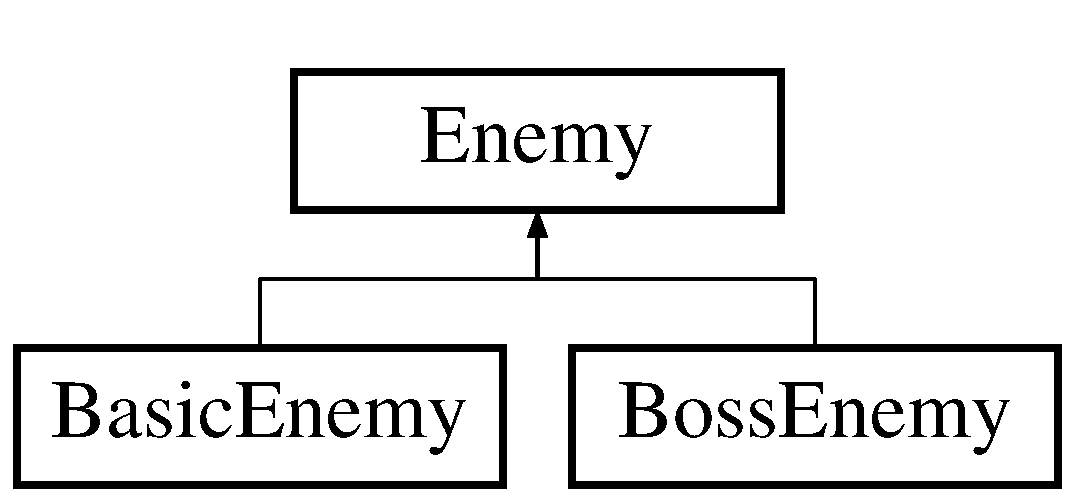
\includegraphics[height=2.000000cm]{class_enemy}
\end{center}
\end{figure}
\subsection*{Slots públicos}
\begin{DoxyCompactItemize}
\item 
virtual void \hyperlink{class_enemy_a1c208ac4a80b892f9692222bcb96f6ae}{move} ()=0
\end{DoxyCompactItemize}
\subsection*{Métodos públicos}
\begin{DoxyCompactItemize}
\item 
\hyperlink{class_enemy_a94f30d348b6d2840fd71675472ba38dd}{Enemy} ()
\end{DoxyCompactItemize}


\subsection{Documentación del constructor y destructor}
\hypertarget{class_enemy_a94f30d348b6d2840fd71675472ba38dd}{}\label{class_enemy_a94f30d348b6d2840fd71675472ba38dd} 
\index{Enemy@{Enemy}!Enemy@{Enemy}}
\index{Enemy@{Enemy}!Enemy@{Enemy}}
\subsubsection{\texorpdfstring{Enemy()}{Enemy()}}
{\footnotesize\ttfamily Enemy\+::\+Enemy (\begin{DoxyParamCaption}{ }\end{DoxyParamCaption})}



\subsection{Documentación de las funciones miembro}
\hypertarget{class_enemy_a1c208ac4a80b892f9692222bcb96f6ae}{}\label{class_enemy_a1c208ac4a80b892f9692222bcb96f6ae} 
\index{Enemy@{Enemy}!move@{move}}
\index{move@{move}!Enemy@{Enemy}}
\subsubsection{\texorpdfstring{move}{move}}
{\footnotesize\ttfamily virtual void Enemy\+::move (\begin{DoxyParamCaption}{ }\end{DoxyParamCaption})\hspace{0.3cm}{\ttfamily [pure virtual]}, {\ttfamily [slot]}}



La documentación para esta clase fue generada a partir de los siguientes ficheros\+:\begin{DoxyCompactItemize}
\item 
\hyperlink{enemy_8h}{enemy.\+h}\item 
\hyperlink{enemy_8cpp}{enemy.\+cpp}\end{DoxyCompactItemize}

\hypertarget{class_enemy_controller}{}\section{Referencia de la Clase Enemy\+Controller}
\label{class_enemy_controller}\index{Enemy\+Controller@{Enemy\+Controller}}


{\ttfamily \#include $<$enemycontroller.\+h$>$}

Diagrama de herencias de Enemy\+Controller\begin{figure}[H]
\begin{center}
\leavevmode
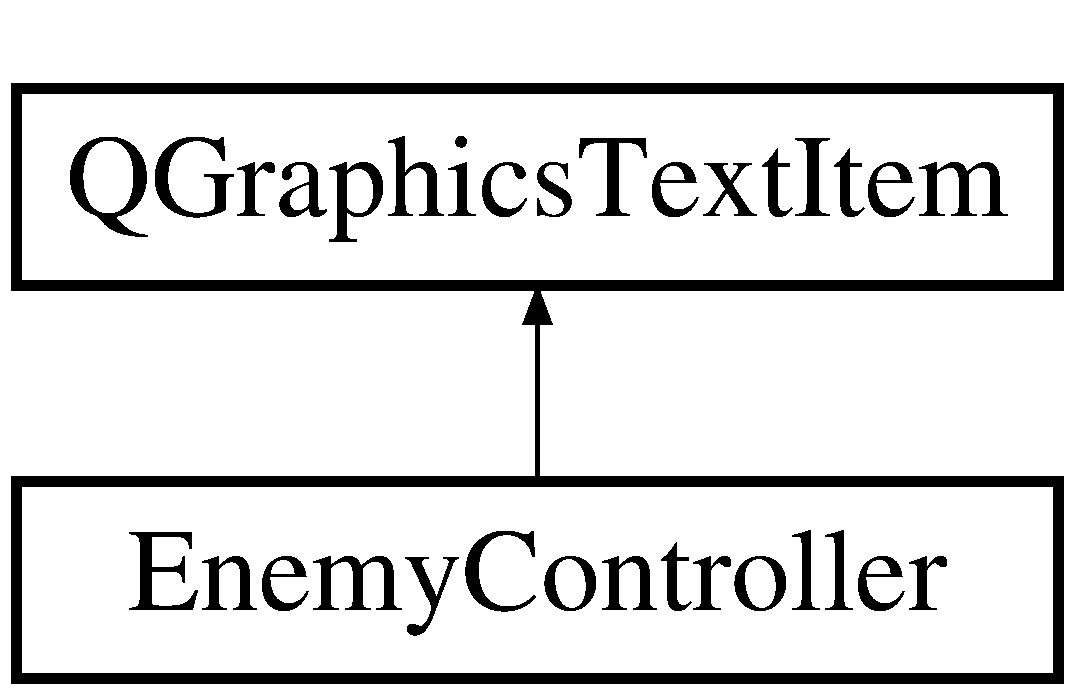
\includegraphics[height=2.000000cm]{class_enemy_controller}
\end{center}
\end{figure}
\subsection*{Métodos públicos}
\begin{DoxyCompactItemize}
\item 
\hyperlink{class_enemy_controller_a9570c4002701ccbabc2bc1609a1f9369}{Enemy\+Controller} (Q\+Graphics\+Text\+Item $\ast$parent=0)
\item 
void \hyperlink{class_enemy_controller_aabdfabc7ce23fb881552c613000bd510}{enemy\+Num\+Decrease} ()
\item 
void \hyperlink{class_enemy_controller_a7ad51104e0e740217a33cbfcc9b94138}{boss\+Live\+Decrease} ()
\item 
int \hyperlink{class_enemy_controller_a8c6a6d2043bbb543a5bf881d662e3e4d}{get\+Enemy\+Num} ()
\item 
int \hyperlink{class_enemy_controller_af5c777646b3431c543e18bba840a30eb}{get\+Boss\+Live} ()
\item 
int \hyperlink{class_enemy_controller_a9c46c7cc4152f83e2b209ef4bceea150}{get\+Vel\+Both} ()
\end{DoxyCompactItemize}


\subsection{Documentación del constructor y destructor}
\hypertarget{class_enemy_controller_a9570c4002701ccbabc2bc1609a1f9369}{}\label{class_enemy_controller_a9570c4002701ccbabc2bc1609a1f9369} 
\index{Enemy\+Controller@{Enemy\+Controller}!Enemy\+Controller@{Enemy\+Controller}}
\index{Enemy\+Controller@{Enemy\+Controller}!Enemy\+Controller@{Enemy\+Controller}}
\subsubsection{\texorpdfstring{Enemy\+Controller()}{EnemyController()}}
{\footnotesize\ttfamily Enemy\+Controller\+::\+Enemy\+Controller (\begin{DoxyParamCaption}\item[{Q\+Graphics\+Text\+Item $\ast$}]{parent = {\ttfamily 0} }\end{DoxyParamCaption})}



\subsection{Documentación de las funciones miembro}
\hypertarget{class_enemy_controller_a7ad51104e0e740217a33cbfcc9b94138}{}\label{class_enemy_controller_a7ad51104e0e740217a33cbfcc9b94138} 
\index{Enemy\+Controller@{Enemy\+Controller}!boss\+Live\+Decrease@{boss\+Live\+Decrease}}
\index{boss\+Live\+Decrease@{boss\+Live\+Decrease}!Enemy\+Controller@{Enemy\+Controller}}
\subsubsection{\texorpdfstring{boss\+Live\+Decrease()}{bossLiveDecrease()}}
{\footnotesize\ttfamily void Enemy\+Controller\+::boss\+Live\+Decrease (\begin{DoxyParamCaption}{ }\end{DoxyParamCaption})}

\hypertarget{class_enemy_controller_aabdfabc7ce23fb881552c613000bd510}{}\label{class_enemy_controller_aabdfabc7ce23fb881552c613000bd510} 
\index{Enemy\+Controller@{Enemy\+Controller}!enemy\+Num\+Decrease@{enemy\+Num\+Decrease}}
\index{enemy\+Num\+Decrease@{enemy\+Num\+Decrease}!Enemy\+Controller@{Enemy\+Controller}}
\subsubsection{\texorpdfstring{enemy\+Num\+Decrease()}{enemyNumDecrease()}}
{\footnotesize\ttfamily void Enemy\+Controller\+::enemy\+Num\+Decrease (\begin{DoxyParamCaption}{ }\end{DoxyParamCaption})}

\hypertarget{class_enemy_controller_af5c777646b3431c543e18bba840a30eb}{}\label{class_enemy_controller_af5c777646b3431c543e18bba840a30eb} 
\index{Enemy\+Controller@{Enemy\+Controller}!get\+Boss\+Live@{get\+Boss\+Live}}
\index{get\+Boss\+Live@{get\+Boss\+Live}!Enemy\+Controller@{Enemy\+Controller}}
\subsubsection{\texorpdfstring{get\+Boss\+Live()}{getBossLive()}}
{\footnotesize\ttfamily int Enemy\+Controller\+::get\+Boss\+Live (\begin{DoxyParamCaption}{ }\end{DoxyParamCaption})}

\hypertarget{class_enemy_controller_a8c6a6d2043bbb543a5bf881d662e3e4d}{}\label{class_enemy_controller_a8c6a6d2043bbb543a5bf881d662e3e4d} 
\index{Enemy\+Controller@{Enemy\+Controller}!get\+Enemy\+Num@{get\+Enemy\+Num}}
\index{get\+Enemy\+Num@{get\+Enemy\+Num}!Enemy\+Controller@{Enemy\+Controller}}
\subsubsection{\texorpdfstring{get\+Enemy\+Num()}{getEnemyNum()}}
{\footnotesize\ttfamily int Enemy\+Controller\+::get\+Enemy\+Num (\begin{DoxyParamCaption}{ }\end{DoxyParamCaption})}

\hypertarget{class_enemy_controller_a9c46c7cc4152f83e2b209ef4bceea150}{}\label{class_enemy_controller_a9c46c7cc4152f83e2b209ef4bceea150} 
\index{Enemy\+Controller@{Enemy\+Controller}!get\+Vel\+Both@{get\+Vel\+Both}}
\index{get\+Vel\+Both@{get\+Vel\+Both}!Enemy\+Controller@{Enemy\+Controller}}
\subsubsection{\texorpdfstring{get\+Vel\+Both()}{getVelBoth()}}
{\footnotesize\ttfamily int Enemy\+Controller\+::get\+Vel\+Both (\begin{DoxyParamCaption}{ }\end{DoxyParamCaption})}



La documentación para esta clase fue generada a partir de los siguientes ficheros\+:\begin{DoxyCompactItemize}
\item 
\hyperlink{enemycontroller_8h}{enemycontroller.\+h}\item 
\hyperlink{enemycontroller_8cpp}{enemycontroller.\+cpp}\end{DoxyCompactItemize}

\hypertarget{class_game}{}\section{Referencia de la Clase Game}
\label{class_game}\index{Game@{Game}}


{\ttfamily \#include $<$game.\+h$>$}

Diagrama de herencias de Game\begin{figure}[H]
\begin{center}
\leavevmode
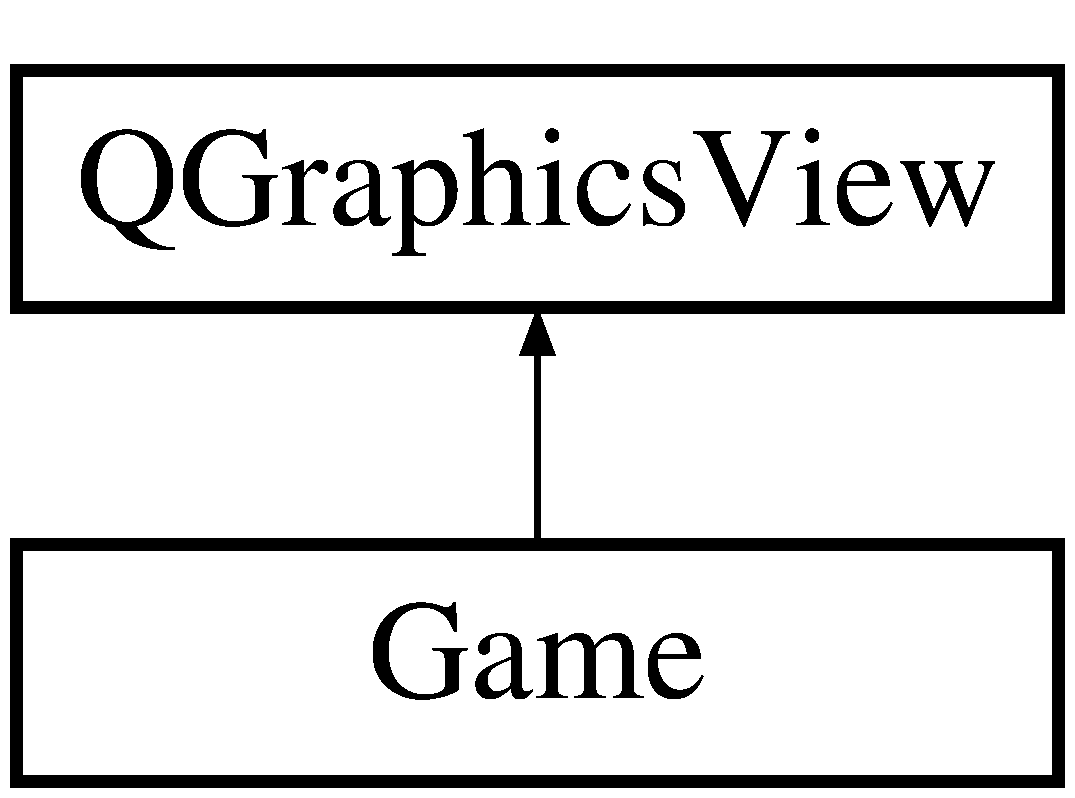
\includegraphics[height=2.000000cm]{class_game}
\end{center}
\end{figure}
\subsection*{Slots públicos}
\begin{DoxyCompactItemize}
\item 
void \hyperlink{class_game_a3d9b98f7c4a96ecf578f75b96c9f0e90}{start} ()
\begin{DoxyCompactList}\small\item\em start is a slot connect with signal clicked \end{DoxyCompactList}\end{DoxyCompactItemize}
\subsection*{Métodos públicos}
\begin{DoxyCompactItemize}
\item 
\hyperlink{class_game_ae3c64a8dd73de0a99849db8ec0e9a86c}{Game} (Q\+Widget $\ast$parent=0)
\item 
void \hyperlink{class_game_af74fd203e3b31917ca9d4769fa608c48}{display\+Main\+Menu} ()
\begin{DoxyCompactList}\small\item\em display\+Main\+Menu show this function with game start \end{DoxyCompactList}\item 
void \hyperlink{class_game_ac7d371f3f30513a4f3c57f521fac9b5f}{game\+Over} ()
\begin{DoxyCompactList}\small\item\em game\+Over function for finish game \end{DoxyCompactList}\item 
void \hyperlink{class_game_a574eb7e3a432099107f3fb3150d2d6ad}{you\+Win} ()
\begin{DoxyCompactList}\small\item\em you\+Win function for finish game \end{DoxyCompactList}\end{DoxyCompactItemize}
\subsection*{Atributos públicos}
\begin{DoxyCompactItemize}
\item 
Q\+Graphics\+Scene $\ast$ \hyperlink{class_game_a8119e3b9a632906c6808fa294b46a92a}{scene}
\item 
\hyperlink{class_player}{Player} $\ast$ \hyperlink{class_game_abec70aa1c0269a9a7e171af4d79e08bf}{player}
\item 
\hyperlink{class_score}{Score} $\ast$ \hyperlink{class_game_ad195acc6b5ee17a5a07fea0b7b4ff5e2}{score}
\item 
\hyperlink{class_healht}{Healht} $\ast$ \hyperlink{class_game_af7860ba10bf58b4bfed1e00f5f699755}{healht}
\item 
\hyperlink{class_basic_enemy}{Basic\+Enemy} $\ast$ \hyperlink{class_game_a14c5877efccfde28a30d4d15f7dd68be}{basic\+Enemy}
\item 
\hyperlink{class_enemy_controller}{Enemy\+Controller} $\ast$ \hyperlink{class_game_a1732035088c7b0150817197895116097}{enemy\+Controller}
\item 
\hyperlink{class_boss_enemy}{Boss\+Enemy} $\ast$ \hyperlink{class_game_a24b3b9175f68e174b9cc88c4372fee68}{boss\+Enemy}
\item 
\hyperlink{class_back_ground}{Back\+Ground} $\ast$ \hyperlink{class_game_a524bd09cf01b51b835f6c574c88ed0ee}{back\+Ground}
\end{DoxyCompactItemize}


\subsection{Documentación del constructor y destructor}
\hypertarget{class_game_ae3c64a8dd73de0a99849db8ec0e9a86c}{}\label{class_game_ae3c64a8dd73de0a99849db8ec0e9a86c} 
\index{Game@{Game}!Game@{Game}}
\index{Game@{Game}!Game@{Game}}
\subsubsection{\texorpdfstring{Game()}{Game()}}
{\footnotesize\ttfamily Game\+::\+Game (\begin{DoxyParamCaption}\item[{Q\+Widget $\ast$}]{parent = {\ttfamily 0} }\end{DoxyParamCaption})}



\subsection{Documentación de las funciones miembro}
\hypertarget{class_game_af74fd203e3b31917ca9d4769fa608c48}{}\label{class_game_af74fd203e3b31917ca9d4769fa608c48} 
\index{Game@{Game}!display\+Main\+Menu@{display\+Main\+Menu}}
\index{display\+Main\+Menu@{display\+Main\+Menu}!Game@{Game}}
\subsubsection{\texorpdfstring{display\+Main\+Menu()}{displayMainMenu()}}
{\footnotesize\ttfamily void Game\+::display\+Main\+Menu (\begin{DoxyParamCaption}{ }\end{DoxyParamCaption})}



display\+Main\+Menu show this function with game start 

\hypertarget{class_game_ac7d371f3f30513a4f3c57f521fac9b5f}{}\label{class_game_ac7d371f3f30513a4f3c57f521fac9b5f} 
\index{Game@{Game}!game\+Over@{game\+Over}}
\index{game\+Over@{game\+Over}!Game@{Game}}
\subsubsection{\texorpdfstring{game\+Over()}{gameOver()}}
{\footnotesize\ttfamily void Game\+::game\+Over (\begin{DoxyParamCaption}{ }\end{DoxyParamCaption})}



game\+Over function for finish game 

\hypertarget{class_game_a3d9b98f7c4a96ecf578f75b96c9f0e90}{}\label{class_game_a3d9b98f7c4a96ecf578f75b96c9f0e90} 
\index{Game@{Game}!start@{start}}
\index{start@{start}!Game@{Game}}
\subsubsection{\texorpdfstring{start}{start}}
{\footnotesize\ttfamily void Game\+::start (\begin{DoxyParamCaption}{ }\end{DoxyParamCaption})\hspace{0.3cm}{\ttfamily [slot]}}



start is a slot connect with signal clicked 

\hypertarget{class_game_a574eb7e3a432099107f3fb3150d2d6ad}{}\label{class_game_a574eb7e3a432099107f3fb3150d2d6ad} 
\index{Game@{Game}!you\+Win@{you\+Win}}
\index{you\+Win@{you\+Win}!Game@{Game}}
\subsubsection{\texorpdfstring{you\+Win()}{youWin()}}
{\footnotesize\ttfamily void Game\+::you\+Win (\begin{DoxyParamCaption}{ }\end{DoxyParamCaption})}



you\+Win function for finish game 



\subsection{Documentación de los datos miembro}
\hypertarget{class_game_a524bd09cf01b51b835f6c574c88ed0ee}{}\label{class_game_a524bd09cf01b51b835f6c574c88ed0ee} 
\index{Game@{Game}!back\+Ground@{back\+Ground}}
\index{back\+Ground@{back\+Ground}!Game@{Game}}
\subsubsection{\texorpdfstring{back\+Ground}{backGround}}
{\footnotesize\ttfamily \hyperlink{class_back_ground}{Back\+Ground}$\ast$ Game\+::back\+Ground}

\hypertarget{class_game_a14c5877efccfde28a30d4d15f7dd68be}{}\label{class_game_a14c5877efccfde28a30d4d15f7dd68be} 
\index{Game@{Game}!basic\+Enemy@{basic\+Enemy}}
\index{basic\+Enemy@{basic\+Enemy}!Game@{Game}}
\subsubsection{\texorpdfstring{basic\+Enemy}{basicEnemy}}
{\footnotesize\ttfamily \hyperlink{class_basic_enemy}{Basic\+Enemy}$\ast$ Game\+::basic\+Enemy}

\hypertarget{class_game_a24b3b9175f68e174b9cc88c4372fee68}{}\label{class_game_a24b3b9175f68e174b9cc88c4372fee68} 
\index{Game@{Game}!boss\+Enemy@{boss\+Enemy}}
\index{boss\+Enemy@{boss\+Enemy}!Game@{Game}}
\subsubsection{\texorpdfstring{boss\+Enemy}{bossEnemy}}
{\footnotesize\ttfamily \hyperlink{class_boss_enemy}{Boss\+Enemy}$\ast$ Game\+::boss\+Enemy}

\hypertarget{class_game_a1732035088c7b0150817197895116097}{}\label{class_game_a1732035088c7b0150817197895116097} 
\index{Game@{Game}!enemy\+Controller@{enemy\+Controller}}
\index{enemy\+Controller@{enemy\+Controller}!Game@{Game}}
\subsubsection{\texorpdfstring{enemy\+Controller}{enemyController}}
{\footnotesize\ttfamily \hyperlink{class_enemy_controller}{Enemy\+Controller}$\ast$ Game\+::enemy\+Controller}

\hypertarget{class_game_af7860ba10bf58b4bfed1e00f5f699755}{}\label{class_game_af7860ba10bf58b4bfed1e00f5f699755} 
\index{Game@{Game}!healht@{healht}}
\index{healht@{healht}!Game@{Game}}
\subsubsection{\texorpdfstring{healht}{healht}}
{\footnotesize\ttfamily \hyperlink{class_healht}{Healht}$\ast$ Game\+::healht}

\hypertarget{class_game_abec70aa1c0269a9a7e171af4d79e08bf}{}\label{class_game_abec70aa1c0269a9a7e171af4d79e08bf} 
\index{Game@{Game}!player@{player}}
\index{player@{player}!Game@{Game}}
\subsubsection{\texorpdfstring{player}{player}}
{\footnotesize\ttfamily \hyperlink{class_player}{Player}$\ast$ Game\+::player}

\hypertarget{class_game_a8119e3b9a632906c6808fa294b46a92a}{}\label{class_game_a8119e3b9a632906c6808fa294b46a92a} 
\index{Game@{Game}!scene@{scene}}
\index{scene@{scene}!Game@{Game}}
\subsubsection{\texorpdfstring{scene}{scene}}
{\footnotesize\ttfamily Q\+Graphics\+Scene$\ast$ Game\+::scene}

\hypertarget{class_game_ad195acc6b5ee17a5a07fea0b7b4ff5e2}{}\label{class_game_ad195acc6b5ee17a5a07fea0b7b4ff5e2} 
\index{Game@{Game}!score@{score}}
\index{score@{score}!Game@{Game}}
\subsubsection{\texorpdfstring{score}{score}}
{\footnotesize\ttfamily \hyperlink{class_score}{Score}$\ast$ Game\+::score}



La documentación para esta clase fue generada a partir de los siguientes ficheros\+:\begin{DoxyCompactItemize}
\item 
\hyperlink{game_8h}{game.\+h}\item 
\hyperlink{game_8cpp}{game.\+cpp}\end{DoxyCompactItemize}

\hypertarget{class_healht}{}\section{Referencia de la Clase Healht}
\label{class_healht}\index{Healht@{Healht}}


{\ttfamily \#include $<$healht.\+h$>$}

Diagrama de herencias de Healht\begin{figure}[H]
\begin{center}
\leavevmode
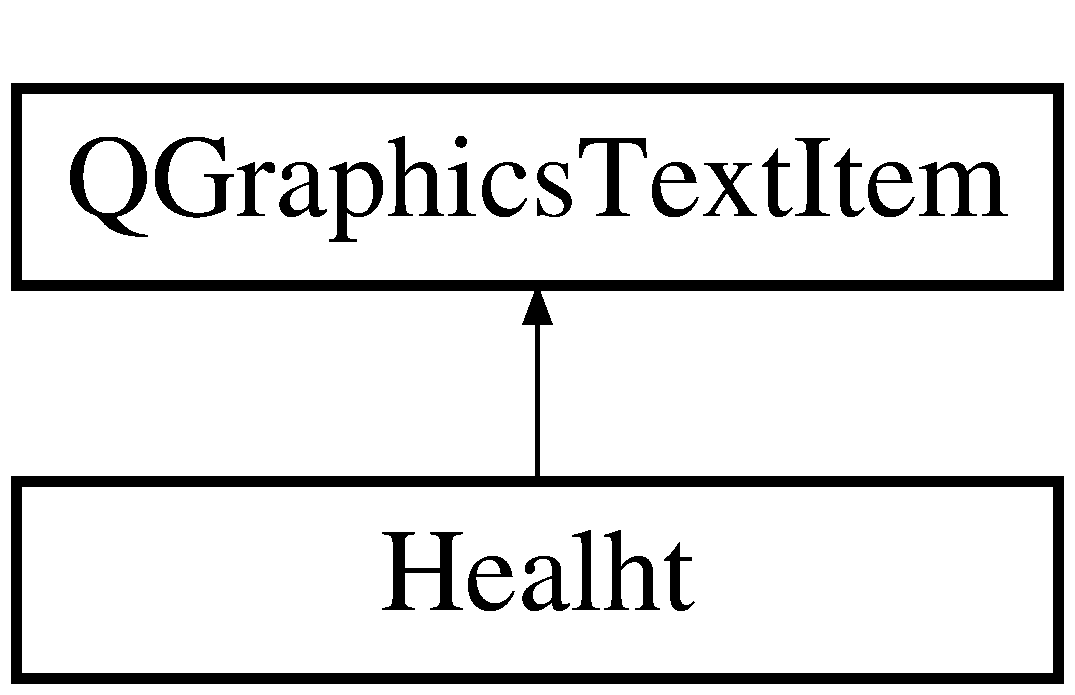
\includegraphics[height=2.000000cm]{class_healht}
\end{center}
\end{figure}
\subsection*{Métodos públicos}
\begin{DoxyCompactItemize}
\item 
\hyperlink{class_healht_ae2cc49ac8d1332e5fc9923839c9f2f5a}{Healht} (Q\+Graphics\+Text\+Item $\ast$parent=0)
\item 
void \hyperlink{class_healht_a287604024264761de0026122d76f5b9d}{decrease} (int n)
\begin{DoxyCompactList}\small\item\em decrease decrease live function \end{DoxyCompactList}\item 
int \hyperlink{class_healht_a7ee67dc2c89fb370bc827cfedc8ae150}{get\+Health} ()
\begin{DoxyCompactList}\small\item\em get\+Health \end{DoxyCompactList}\end{DoxyCompactItemize}


\subsection{Documentación del constructor y destructor}
\hypertarget{class_healht_ae2cc49ac8d1332e5fc9923839c9f2f5a}{}\label{class_healht_ae2cc49ac8d1332e5fc9923839c9f2f5a} 
\index{Healht@{Healht}!Healht@{Healht}}
\index{Healht@{Healht}!Healht@{Healht}}
\subsubsection{\texorpdfstring{Healht()}{Healht()}}
{\footnotesize\ttfamily Healht\+::\+Healht (\begin{DoxyParamCaption}\item[{Q\+Graphics\+Text\+Item $\ast$}]{parent = {\ttfamily 0} }\end{DoxyParamCaption})}



\subsection{Documentación de las funciones miembro}
\hypertarget{class_healht_a287604024264761de0026122d76f5b9d}{}\label{class_healht_a287604024264761de0026122d76f5b9d} 
\index{Healht@{Healht}!decrease@{decrease}}
\index{decrease@{decrease}!Healht@{Healht}}
\subsubsection{\texorpdfstring{decrease()}{decrease()}}
{\footnotesize\ttfamily void Healht\+::decrease (\begin{DoxyParamCaption}\item[{int}]{n }\end{DoxyParamCaption})}



decrease decrease live function 


\begin{DoxyParams}{Parámetros}
{\em n} & n is a number for decrease live \\
\hline
\end{DoxyParams}
\hypertarget{class_healht_a7ee67dc2c89fb370bc827cfedc8ae150}{}\label{class_healht_a7ee67dc2c89fb370bc827cfedc8ae150} 
\index{Healht@{Healht}!get\+Health@{get\+Health}}
\index{get\+Health@{get\+Health}!Healht@{Healht}}
\subsubsection{\texorpdfstring{get\+Health()}{getHealth()}}
{\footnotesize\ttfamily int Healht\+::get\+Health (\begin{DoxyParamCaption}{ }\end{DoxyParamCaption})\hspace{0.3cm}{\ttfamily [inline]}}



get\+Health 

\begin{DoxyReturn}{Devuelve}
return player live 
\end{DoxyReturn}


La documentación para esta clase fue generada a partir de los siguientes ficheros\+:\begin{DoxyCompactItemize}
\item 
\hyperlink{healht_8h}{healht.\+h}\item 
\hyperlink{healht_8cpp}{healht.\+cpp}\end{DoxyCompactItemize}

\hypertarget{class_player}{}\section{Referencia de la Clase Player}
\label{class_player}\index{Player@{Player}}


{\ttfamily \#include $<$player.\+h$>$}

Diagrama de herencias de Player\begin{figure}[H]
\begin{center}
\leavevmode
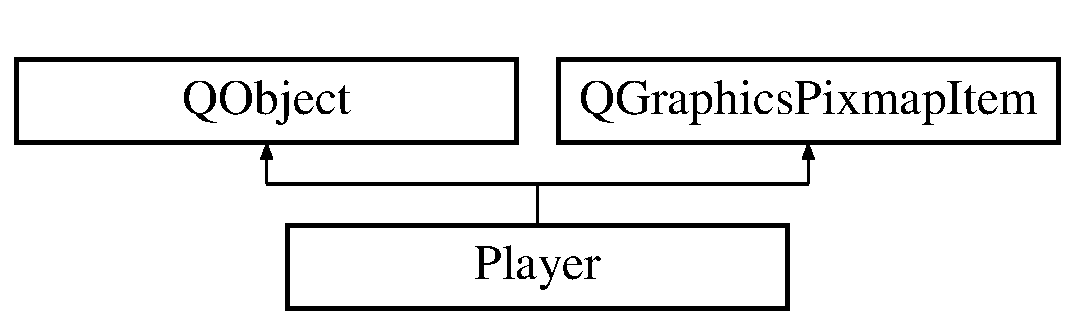
\includegraphics[height=2.000000cm]{class_player}
\end{center}
\end{figure}
\subsection*{Slots públicos}
\begin{DoxyCompactItemize}
\item 
void \hyperlink{class_player_a59ae3f2c7151032a85e58b1591cad769}{spawn} ()
\begin{DoxyCompactList}\small\item\em spawn is a slot \end{DoxyCompactList}\end{DoxyCompactItemize}
\subsection*{Métodos públicos}
\begin{DoxyCompactItemize}
\item 
\hyperlink{class_player_affe0cc3cb714f6deb4e62f0c0d3f1fd8}{Player} ()
\item 
void \hyperlink{class_player_a4d269c4118c29b0ee85c1e0f674260ee}{key\+Press\+Event} (Q\+Key\+Event $\ast$event)
\begin{DoxyCompactList}\small\item\em key\+Press\+Event \end{DoxyCompactList}\end{DoxyCompactItemize}


\subsection{Documentación del constructor y destructor}
\hypertarget{class_player_affe0cc3cb714f6deb4e62f0c0d3f1fd8}{}\label{class_player_affe0cc3cb714f6deb4e62f0c0d3f1fd8} 
\index{Player@{Player}!Player@{Player}}
\index{Player@{Player}!Player@{Player}}
\subsubsection{\texorpdfstring{Player()}{Player()}}
{\footnotesize\ttfamily Player\+::\+Player (\begin{DoxyParamCaption}{ }\end{DoxyParamCaption})}



\subsection{Documentación de las funciones miembro}
\hypertarget{class_player_a4d269c4118c29b0ee85c1e0f674260ee}{}\label{class_player_a4d269c4118c29b0ee85c1e0f674260ee} 
\index{Player@{Player}!key\+Press\+Event@{key\+Press\+Event}}
\index{key\+Press\+Event@{key\+Press\+Event}!Player@{Player}}
\subsubsection{\texorpdfstring{key\+Press\+Event()}{keyPressEvent()}}
{\footnotesize\ttfamily void Player\+::key\+Press\+Event (\begin{DoxyParamCaption}\item[{Q\+Key\+Event $\ast$}]{event }\end{DoxyParamCaption})}



key\+Press\+Event 


\begin{DoxyParams}{Parámetros}
{\em event} & if you press a key \\
\hline
\end{DoxyParams}
\hypertarget{class_player_a59ae3f2c7151032a85e58b1591cad769}{}\label{class_player_a59ae3f2c7151032a85e58b1591cad769} 
\index{Player@{Player}!spawn@{spawn}}
\index{spawn@{spawn}!Player@{Player}}
\subsubsection{\texorpdfstring{spawn}{spawn}}
{\footnotesize\ttfamily void Player\+::spawn (\begin{DoxyParamCaption}{ }\end{DoxyParamCaption})\hspace{0.3cm}{\ttfamily [slot]}}



spawn is a slot 



La documentación para esta clase fue generada a partir de los siguientes ficheros\+:\begin{DoxyCompactItemize}
\item 
\hyperlink{player_8h}{player.\+h}\item 
\hyperlink{player_8cpp}{player.\+cpp}\end{DoxyCompactItemize}

\hypertarget{class_score}{}\section{Referencia de la Clase Score}
\label{class_score}\index{Score@{Score}}


{\ttfamily \#include $<$score.\+h$>$}

Diagrama de herencias de Score\begin{figure}[H]
\begin{center}
\leavevmode
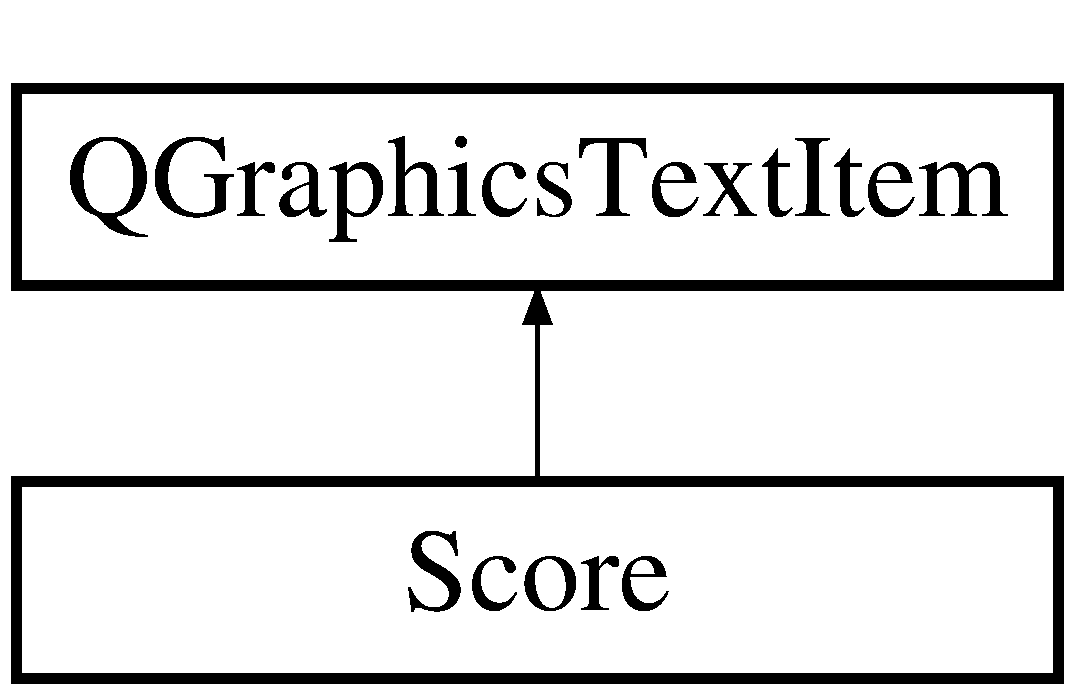
\includegraphics[height=2.000000cm]{class_score}
\end{center}
\end{figure}
\subsection*{Métodos públicos}
\begin{DoxyCompactItemize}
\item 
\hyperlink{class_score_af7c3392a27388a66b8a94448a995634d}{Score} (Q\+Graphics\+Item $\ast$parent=0)
\item 
void \hyperlink{class_score_ab5dbfab6935903c075509546878cfbda}{increase} ()
\item 
int \hyperlink{class_score_a8627c93270c188a3fd28a25b1d07a9e7}{get\+Score} ()
\begin{DoxyCompactList}\small\item\em get\+Score \end{DoxyCompactList}\item 
void \hyperlink{class_score_a4ed969e7c03d43036b1800b9ac9d224f}{set\+Score} (int n)
\begin{DoxyCompactList}\small\item\em set\+Score \end{DoxyCompactList}\end{DoxyCompactItemize}


\subsection{Documentación del constructor y destructor}
\hypertarget{class_score_af7c3392a27388a66b8a94448a995634d}{}\label{class_score_af7c3392a27388a66b8a94448a995634d} 
\index{Score@{Score}!Score@{Score}}
\index{Score@{Score}!Score@{Score}}
\subsubsection{\texorpdfstring{Score()}{Score()}}
{\footnotesize\ttfamily Score\+::\+Score (\begin{DoxyParamCaption}\item[{Q\+Graphics\+Item $\ast$}]{parent = {\ttfamily 0} }\end{DoxyParamCaption})}



\subsection{Documentación de las funciones miembro}
\hypertarget{class_score_a8627c93270c188a3fd28a25b1d07a9e7}{}\label{class_score_a8627c93270c188a3fd28a25b1d07a9e7} 
\index{Score@{Score}!get\+Score@{get\+Score}}
\index{get\+Score@{get\+Score}!Score@{Score}}
\subsubsection{\texorpdfstring{get\+Score()}{getScore()}}
{\footnotesize\ttfamily int Score\+::get\+Score (\begin{DoxyParamCaption}{ }\end{DoxyParamCaption})\hspace{0.3cm}{\ttfamily [inline]}}



get\+Score 

\begin{DoxyReturn}{Devuelve}
return score 
\end{DoxyReturn}
\hypertarget{class_score_ab5dbfab6935903c075509546878cfbda}{}\label{class_score_ab5dbfab6935903c075509546878cfbda} 
\index{Score@{Score}!increase@{increase}}
\index{increase@{increase}!Score@{Score}}
\subsubsection{\texorpdfstring{increase()}{increase()}}
{\footnotesize\ttfamily void Score\+::increase (\begin{DoxyParamCaption}{ }\end{DoxyParamCaption})}

\hypertarget{class_score_a4ed969e7c03d43036b1800b9ac9d224f}{}\label{class_score_a4ed969e7c03d43036b1800b9ac9d224f} 
\index{Score@{Score}!set\+Score@{set\+Score}}
\index{set\+Score@{set\+Score}!Score@{Score}}
\subsubsection{\texorpdfstring{set\+Score()}{setScore()}}
{\footnotesize\ttfamily void Score\+::set\+Score (\begin{DoxyParamCaption}\item[{int}]{n }\end{DoxyParamCaption})\hspace{0.3cm}{\ttfamily [inline]}}



set\+Score 


\begin{DoxyParams}{Parámetros}
{\em n} & is new val for score \\
\hline
\end{DoxyParams}


La documentación para esta clase fue generada a partir de los siguientes ficheros\+:\begin{DoxyCompactItemize}
\item 
\hyperlink{score_8h}{score.\+h}\item 
\hyperlink{score_8cpp}{score.\+cpp}\end{DoxyCompactItemize}

\chapter{Documentación de archivos}
\hypertarget{background_8cpp}{}\section{Referencia del Archivo background.\+cpp}
\label{background_8cpp}\index{background.\+cpp@{background.\+cpp}}
{\ttfamily \#include \char`\"{}background.\+h\char`\"{}}\newline

\hypertarget{background_8h}{}\section{Referencia del Archivo background.\+h}
\label{background_8h}\index{background.\+h@{background.\+h}}


this class is for place the image background at star of the game  


{\ttfamily \#include $<$Q\+Graphics\+Path\+Item$>$}\newline
\subsection*{Clases}
\begin{DoxyCompactItemize}
\item 
class \hyperlink{class_back_ground}{Back\+Ground}
\end{DoxyCompactItemize}


\subsection{Descripción detallada}
this class is for place the image background at star of the game 

\begin{DoxyVersion}{Versión}
1.\+0 
\end{DoxyVersion}
\begin{DoxyDate}{Fecha}
25/12/16 
\end{DoxyDate}
\begin{DoxyAuthor}{Autor}
Raul Edgar Quispe Totocayo  class background 
\end{DoxyAuthor}

\hypertarget{basicenemy_8cpp}{}\section{Referencia del Archivo basicenemy.\+cpp}
\label{basicenemy_8cpp}\index{basicenemy.\+cpp@{basicenemy.\+cpp}}
{\ttfamily \#include \char`\"{}basicenemy.\+h\char`\"{}}\newline
{\ttfamily \#include $<$Q\+Graphics\+Scene$>$}\newline
{\ttfamily \#include $<$Q\+Debug$>$}\newline
{\ttfamily \#include $<$Q\+Timer$>$}\newline
{\ttfamily \#include $<$Q\+List$>$}\newline
{\ttfamily \#include $<$typeinfo$>$}\newline
{\ttfamily \#include $<$iostream$>$}\newline
{\ttfamily \#include $<$random$>$}\newline
{\ttfamily \#include $<$ctime$>$}\newline
{\ttfamily \#include $<$iomanip$>$}\newline
{\ttfamily \#include $<$stdlib.\+h$>$}\newline

\hypertarget{basicenemy_8h}{}\section{Referencia del Archivo basicenemy.\+h}
\label{basicenemy_8h}\index{basicenemy.\+h@{basicenemy.\+h}}


this class is to representation of basic enemy if you killed basic enemy you score increase if you score is more of 10 your live increase in 50  


{\ttfamily \#include \char`\"{}enemy.\+h\char`\"{}}\newline
{\ttfamily \#include $<$Q\+Object$>$}\newline
{\ttfamily \#include $<$Q\+Graphics\+Pixmap\+Item$>$}\newline
\subsection*{Clases}
\begin{DoxyCompactItemize}
\item 
class \hyperlink{class_basic_enemy}{Basic\+Enemy}
\end{DoxyCompactItemize}


\subsection{Descripción detallada}
this class is to representation of basic enemy if you killed basic enemy you score increase if you score is more of 10 your live increase in 50 

\begin{DoxyVersion}{Versión}
1.\+0 
\end{DoxyVersion}
\begin{DoxyDate}{Fecha}
25/12/16 
\end{DoxyDate}
\begin{DoxyAuthor}{Autor}
Raul Edgar Quispe Totocayo  basic enemy 
\end{DoxyAuthor}

\hypertarget{bossenemy_8cpp}{}\section{Referencia del Archivo bossenemy.\+cpp}
\label{bossenemy_8cpp}\index{bossenemy.\+cpp@{bossenemy.\+cpp}}
{\ttfamily \#include \char`\"{}game.\+h\char`\"{}}\newline
{\ttfamily \#include \char`\"{}bossenemy.\+h\char`\"{}}\newline
{\ttfamily \#include $<$Q\+Graphics\+Scene$>$}\newline
{\ttfamily \#include $<$Q\+Debug$>$}\newline
{\ttfamily \#include $<$Q\+Timer$>$}\newline
{\ttfamily \#include $<$Q\+List$>$}\newline
{\ttfamily \#include $<$typeinfo$>$}\newline
{\ttfamily \#include $<$iostream$>$}\newline
{\ttfamily \#include $<$random$>$}\newline
{\ttfamily \#include $<$ctime$>$}\newline
{\ttfamily \#include $<$iomanip$>$}\newline
{\ttfamily \#include $<$stdlib.\+h$>$}\newline
\subsection*{Variables}
\begin{DoxyCompactItemize}
\item 
\hyperlink{class_game}{Game} $\ast$ \hyperlink{bossenemy_8cpp_a58bdb5643d0814ac4e697a1564b79b70}{game}
\end{DoxyCompactItemize}


\subsection{Documentación de las variables}
\hypertarget{bossenemy_8cpp_a58bdb5643d0814ac4e697a1564b79b70}{}\label{bossenemy_8cpp_a58bdb5643d0814ac4e697a1564b79b70} 
\index{bossenemy.\+cpp@{bossenemy.\+cpp}!game@{game}}
\index{game@{game}!bossenemy.\+cpp@{bossenemy.\+cpp}}
\subsubsection{\texorpdfstring{game}{game}}
{\footnotesize\ttfamily \hyperlink{class_game}{Game}$\ast$ game}


\hypertarget{bossenemy_8h}{}\section{Referencia del Archivo bossenemy.\+h}
\label{bossenemy_8h}\index{bossenemy.\+h@{bossenemy.\+h}}


this class is toa representation a boss enemy if you killed a boss enemy you win the game  


{\ttfamily \#include \char`\"{}enemy.\+h\char`\"{}}\newline
{\ttfamily \#include $<$Q\+Object$>$}\newline
{\ttfamily \#include $<$Q\+Graphics\+Pixmap\+Item$>$}\newline
\subsection*{Clases}
\begin{DoxyCompactItemize}
\item 
class \hyperlink{class_boss_enemy}{Boss\+Enemy}
\end{DoxyCompactItemize}


\subsection{Descripción detallada}
this class is toa representation a boss enemy if you killed a boss enemy you win the game 

\begin{DoxyVersion}{Versión}
1.\+0 
\end{DoxyVersion}
\begin{DoxyDate}{Fecha}
25/12/16 
\end{DoxyDate}
\begin{DoxyAuthor}{Autor}
Raul Edgar Quispe Totocayo  class \hyperlink{class_boss_enemy}{Boss\+Enemy} 
\end{DoxyAuthor}

\hypertarget{bullet_8cpp}{}\section{Referencia del Archivo bullet.\+cpp}
\label{bullet_8cpp}\index{bullet.\+cpp@{bullet.\+cpp}}
{\ttfamily \#include \char`\"{}bullet.\+h\char`\"{}}\newline
{\ttfamily \#include \char`\"{}game.\+h\char`\"{}}\newline
{\ttfamily \#include \char`\"{}basicenemy.\+h\char`\"{}}\newline
{\ttfamily \#include \char`\"{}bossenemy.\+h\char`\"{}}\newline
{\ttfamily \#include $<$Q\+Timer$>$}\newline
{\ttfamily \#include $<$Q\+Debug$>$}\newline
{\ttfamily \#include $<$Q\+Graphics\+Scene$>$}\newline
{\ttfamily \#include $<$Q\+List$>$}\newline
{\ttfamily \#include $<$typeinfo$>$}\newline
\subsection*{Variables}
\begin{DoxyCompactItemize}
\item 
\hyperlink{class_game}{Game} $\ast$ \hyperlink{bullet_8cpp_a58bdb5643d0814ac4e697a1564b79b70}{game}
\end{DoxyCompactItemize}


\subsection{Documentación de las variables}
\hypertarget{bullet_8cpp_a58bdb5643d0814ac4e697a1564b79b70}{}\label{bullet_8cpp_a58bdb5643d0814ac4e697a1564b79b70} 
\index{bullet.\+cpp@{bullet.\+cpp}!game@{game}}
\index{game@{game}!bullet.\+cpp@{bullet.\+cpp}}
\subsubsection{\texorpdfstring{game}{game}}
{\footnotesize\ttfamily \hyperlink{class_game}{Game}$\ast$ game}


\hypertarget{bullet_8h}{}\section{Referencia del Archivo bullet.\+h}
\label{bullet_8h}\index{bullet.\+h@{bullet.\+h}}
{\ttfamily \#include $<$Q\+Graphics\+Pixmap\+Item$>$}\newline
{\ttfamily \#include $<$Q\+Object$>$}\newline
\subsection*{Clases}
\begin{DoxyCompactItemize}
\item 
class \hyperlink{class_bullet}{Bullet}
\end{DoxyCompactItemize}


\subsection{Descripción detallada}
\begin{DoxyVersion}{Versión}
1.\+0 
\end{DoxyVersion}
\begin{DoxyDate}{Fecha}
25/12/16 
\end{DoxyDate}
\begin{DoxyAuthor}{Autor}
Raul Edgar Quispe Totocayo  class bullet 
\end{DoxyAuthor}

\hypertarget{button_8cpp}{}\section{Referencia del Archivo button.\+cpp}
\label{button_8cpp}\index{button.\+cpp@{button.\+cpp}}
{\ttfamily \#include \char`\"{}button.\+h\char`\"{}}\newline
{\ttfamily \#include $<$Q\+Graphics\+Text\+Item$>$}\newline
{\ttfamily \#include $<$Q\+Brush$>$}\newline

\hypertarget{button_8h}{}\section{Referencia del Archivo button.\+h}
\label{button_8h}\index{button.\+h@{button.\+h}}


this class is for create button for start or quit of the game  


{\ttfamily \#include $<$Q\+Graphics\+Rect\+Item$>$}\newline
{\ttfamily \#include $<$Q\+Graphics\+Scene\+Mouse\+Event$>$}\newline
\subsection*{Clases}
\begin{DoxyCompactItemize}
\item 
class \hyperlink{class_button}{Button}
\end{DoxyCompactItemize}


\subsection{Descripción detallada}
this class is for create button for start or quit of the game 

\begin{DoxyVersion}{Versión}
1.\+0 
\end{DoxyVersion}
\begin{DoxyDate}{Fecha}
25/12/16 
\end{DoxyDate}
\begin{DoxyAuthor}{Autor}
Raul Edgar Quispe Totocayo  class button 
\end{DoxyAuthor}

\hypertarget{enemy_8cpp}{}\section{Referencia del Archivo enemy.\+cpp}
\label{enemy_8cpp}\index{enemy.\+cpp@{enemy.\+cpp}}
{\ttfamily \#include \char`\"{}enemy.\+h\char`\"{}}\newline
{\ttfamily \#include $<$iostream$>$}\newline

\hypertarget{enemy_8h}{}\section{Referencia del Archivo enemy.\+h}
\label{enemy_8h}\index{enemy.\+h@{enemy.\+h}}
{\ttfamily \#include $<$Q\+Object$>$}\newline
\subsection*{Clases}
\begin{DoxyCompactItemize}
\item 
class \hyperlink{class_enemy}{Enemy}
\end{DoxyCompactItemize}


\subsection{Descripción detallada}
\begin{DoxyVersion}{Versión}
1.\+0 
\end{DoxyVersion}
\begin{DoxyDate}{Fecha}
25/12/16 
\end{DoxyDate}
\begin{DoxyAuthor}{Autor}
Raul Edgar Quispe Totocayo  abstract class enemy 
\end{DoxyAuthor}

\hypertarget{enemycontroller_8cpp}{}\section{Referencia del Archivo enemycontroller.\+cpp}
\label{enemycontroller_8cpp}\index{enemycontroller.\+cpp@{enemycontroller.\+cpp}}
{\ttfamily \#include \char`\"{}enemycontroller.\+h\char`\"{}}\newline
{\ttfamily \#include $<$Q\+Font$>$}\newline
{\ttfamily \#include $<$Q\+Debug$>$}\newline

\hypertarget{enemycontroller_8h}{}\section{Referencia del Archivo enemycontroller.\+h}
\label{enemycontroller_8h}\index{enemycontroller.\+h@{enemycontroller.\+h}}


this class is for controller enemy for exmaple to control your live or number enemies  


{\ttfamily \#include $<$Q\+Graphics\+Text\+Item$>$}\newline
\subsection*{Clases}
\begin{DoxyCompactItemize}
\item 
class \hyperlink{class_enemy_controller}{Enemy\+Controller}
\end{DoxyCompactItemize}


\subsection{Descripción detallada}
this class is for controller enemy for exmaple to control your live or number enemies 

\begin{DoxyVersion}{Versión}
1.\+0 
\end{DoxyVersion}
\begin{DoxyDate}{Fecha}
25/12/16 
\end{DoxyDate}
\begin{DoxyAuthor}{Autor}
Raul Edgar Quispe Totocayo  class enemycontroller 
\end{DoxyAuthor}

\hypertarget{game_8cpp}{}\section{Referencia del Archivo game.\+cpp}
\label{game_8cpp}\index{game.\+cpp@{game.\+cpp}}
{\ttfamily \#include \char`\"{}game.\+h\char`\"{}}\newline
{\ttfamily \#include \char`\"{}healht.\+h\char`\"{}}\newline
{\ttfamily \#include \char`\"{}basicenemy.\+h\char`\"{}}\newline
{\ttfamily \#include \char`\"{}button.\+h\char`\"{}}\newline
{\ttfamily \#include $<$Q\+Debug$>$}\newline
{\ttfamily \#include $<$Q\+Timer$>$}\newline
{\ttfamily \#include $<$Q\+Graphics\+Text\+Item$>$}\newline
{\ttfamily \#include $<$Q\+Font$>$}\newline
{\ttfamily \#include $<$Q\+Image$>$}\newline

\hypertarget{game_8h}{}\section{Referencia del Archivo game.\+h}
\label{game_8h}\index{game.\+h@{game.\+h}}
{\ttfamily \#include \char`\"{}score.\+h\char`\"{}}\newline
{\ttfamily \#include \char`\"{}bossenemy.\+h\char`\"{}}\newline
{\ttfamily \#include \char`\"{}basicenemy.\+h\char`\"{}}\newline
{\ttfamily \#include \char`\"{}player.\+h\char`\"{}}\newline
{\ttfamily \#include \char`\"{}bullet.\+h\char`\"{}}\newline
{\ttfamily \#include \char`\"{}healht.\+h\char`\"{}}\newline
{\ttfamily \#include \char`\"{}enemycontroller.\+h\char`\"{}}\newline
{\ttfamily \#include \char`\"{}background.\+h\char`\"{}}\newline
{\ttfamily \#include $<$Q\+Graphics\+Scene$>$}\newline
{\ttfamily \#include $<$Q\+Graphics\+View$>$}\newline
{\ttfamily \#include $<$Q\+Graphics\+Widget$>$}\newline
{\ttfamily \#include $<$Q\+Graphics\+Text\+Item$>$}\newline
\subsection*{Clases}
\begin{DoxyCompactItemize}
\item 
class \hyperlink{class_game}{Game}
\end{DoxyCompactItemize}


\subsection{Descripción detallada}
\begin{DoxyVersion}{Versión}
1.\+0 
\end{DoxyVersion}
\begin{DoxyDate}{Fecha}
25/12/16 
\end{DoxyDate}
\begin{DoxyAuthor}{Autor}
Raul Edgar Quispe Totocayo  class game 
\end{DoxyAuthor}

\hypertarget{healht_8cpp}{}\section{Referencia del Archivo healht.\+cpp}
\label{healht_8cpp}\index{healht.\+cpp@{healht.\+cpp}}
{\ttfamily \#include \char`\"{}healht.\+h\char`\"{}}\newline
{\ttfamily \#include $<$Q\+Font$>$}\newline
{\ttfamily \#include \char`\"{}game.\+h\char`\"{}}\newline
{\ttfamily \#include $<$Q\+Debug$>$}\newline
\subsection*{Variables}
\begin{DoxyCompactItemize}
\item 
\hyperlink{class_game}{Game} $\ast$ \hyperlink{healht_8cpp_a58bdb5643d0814ac4e697a1564b79b70}{game}
\end{DoxyCompactItemize}


\subsection{Documentación de las variables}
\hypertarget{healht_8cpp_a58bdb5643d0814ac4e697a1564b79b70}{}\label{healht_8cpp_a58bdb5643d0814ac4e697a1564b79b70} 
\index{healht.\+cpp@{healht.\+cpp}!game@{game}}
\index{game@{game}!healht.\+cpp@{healht.\+cpp}}
\subsubsection{\texorpdfstring{game}{game}}
{\footnotesize\ttfamily \hyperlink{class_game}{Game}$\ast$ game}


\hypertarget{healht_8h}{}\section{Referencia del Archivo healht.\+h}
\label{healht_8h}\index{healht.\+h@{healht.\+h}}
{\ttfamily \#include $<$Q\+Graphics\+Text\+Item$>$}\newline
\subsection*{Clases}
\begin{DoxyCompactItemize}
\item 
class \hyperlink{class_healht}{Healht}
\end{DoxyCompactItemize}

\hypertarget{main_8cpp}{}\section{Referencia del Archivo main.\+cpp}
\label{main_8cpp}\index{main.\+cpp@{main.\+cpp}}
{\ttfamily \#include $<$Q\+Application$>$}\newline
{\ttfamily \#include \char`\"{}game.\+h\char`\"{}}\newline
\subsection*{Funciones}
\begin{DoxyCompactItemize}
\item 
int \hyperlink{main_8cpp_a0ddf1224851353fc92bfbff6f499fa97}{main} (int argc, char $\ast$argv\mbox{[}$\,$\mbox{]})
\end{DoxyCompactItemize}
\subsection*{Variables}
\begin{DoxyCompactItemize}
\item 
\hyperlink{class_game}{Game} $\ast$ \hyperlink{main_8cpp_a58bdb5643d0814ac4e697a1564b79b70}{game}
\end{DoxyCompactItemize}


\subsection{Documentación de las funciones}
\hypertarget{main_8cpp_a0ddf1224851353fc92bfbff6f499fa97}{}\label{main_8cpp_a0ddf1224851353fc92bfbff6f499fa97} 
\index{main.\+cpp@{main.\+cpp}!main@{main}}
\index{main@{main}!main.\+cpp@{main.\+cpp}}
\subsubsection{\texorpdfstring{main()}{main()}}
{\footnotesize\ttfamily int main (\begin{DoxyParamCaption}\item[{int}]{argc,  }\item[{char $\ast$}]{argv\mbox{[}$\,$\mbox{]} }\end{DoxyParamCaption})}



\subsection{Documentación de las variables}
\hypertarget{main_8cpp_a58bdb5643d0814ac4e697a1564b79b70}{}\label{main_8cpp_a58bdb5643d0814ac4e697a1564b79b70} 
\index{main.\+cpp@{main.\+cpp}!game@{game}}
\index{game@{game}!main.\+cpp@{main.\+cpp}}
\subsubsection{\texorpdfstring{game}{game}}
{\footnotesize\ttfamily \hyperlink{class_game}{Game}$\ast$ game}


\hypertarget{player_8cpp}{}\section{Referencia del Archivo player.\+cpp}
\label{player_8cpp}\index{player.\+cpp@{player.\+cpp}}
{\ttfamily \#include \char`\"{}player.\+h\char`\"{}}\newline
{\ttfamily \#include \char`\"{}bullet.\+h\char`\"{}}\newline
{\ttfamily \#include \char`\"{}game.\+h\char`\"{}}\newline
{\ttfamily \#include \char`\"{}basicenemy.\+h\char`\"{}}\newline
{\ttfamily \#include \char`\"{}bossenemy.\+h\char`\"{}}\newline
{\ttfamily \#include $<$Q\+Key\+Event$>$}\newline
{\ttfamily \#include $<$Q\+Debug$>$}\newline
\subsection*{Variables}
\begin{DoxyCompactItemize}
\item 
\hyperlink{class_game}{Game} $\ast$ \hyperlink{player_8cpp_a58bdb5643d0814ac4e697a1564b79b70}{game}
\item 
int \hyperlink{player_8cpp_a786f1108c99c252dc1afb972c0e06622}{velocidad} = 20
\end{DoxyCompactItemize}


\subsection{Documentación de las variables}
\hypertarget{player_8cpp_a58bdb5643d0814ac4e697a1564b79b70}{}\label{player_8cpp_a58bdb5643d0814ac4e697a1564b79b70} 
\index{player.\+cpp@{player.\+cpp}!game@{game}}
\index{game@{game}!player.\+cpp@{player.\+cpp}}
\subsubsection{\texorpdfstring{game}{game}}
{\footnotesize\ttfamily \hyperlink{class_game}{Game}$\ast$ game}

\hypertarget{player_8cpp_a786f1108c99c252dc1afb972c0e06622}{}\label{player_8cpp_a786f1108c99c252dc1afb972c0e06622} 
\index{player.\+cpp@{player.\+cpp}!velocidad@{velocidad}}
\index{velocidad@{velocidad}!player.\+cpp@{player.\+cpp}}
\subsubsection{\texorpdfstring{velocidad}{velocidad}}
{\footnotesize\ttfamily int velocidad = 20}


\hypertarget{player_8h}{}\section{Referencia del Archivo player.\+h}
\label{player_8h}\index{player.\+h@{player.\+h}}
{\ttfamily \#include $<$Q\+Graphics\+Scene$>$}\newline
{\ttfamily \#include $<$Q\+Graphics\+Pixmap\+Item$>$}\newline
{\ttfamily \#include $<$Q\+Key\+Event$>$}\newline
{\ttfamily \#include $<$Q\+Object$>$}\newline
\subsection*{Clases}
\begin{DoxyCompactItemize}
\item 
class \hyperlink{class_player}{Player}
\end{DoxyCompactItemize}


\subsection{Descripción detallada}
\begin{DoxyVersion}{Versión}
1.\+0 
\end{DoxyVersion}
\begin{DoxyDate}{Fecha}
25/12/16 
\end{DoxyDate}
\begin{DoxyAuthor}{Autor}
Raul Edgar Quispe Totocayo  class player 
\end{DoxyAuthor}

\hypertarget{score_8cpp}{}\section{Referencia del Archivo score.\+cpp}
\label{score_8cpp}\index{score.\+cpp@{score.\+cpp}}
{\ttfamily \#include \char`\"{}score.\+h\char`\"{}}\newline
{\ttfamily \#include $<$Q\+Font$>$}\newline

\hypertarget{score_8h}{}\section{Referencia del Archivo score.\+h}
\label{score_8h}\index{score.\+h@{score.\+h}}
{\ttfamily \#include $<$Q\+Graphics\+Text\+Item$>$}\newline
\subsection*{Clases}
\begin{DoxyCompactItemize}
\item 
class \hyperlink{class_score}{Score}
\end{DoxyCompactItemize}


\subsection{Descripción detallada}
\begin{DoxyVersion}{Versión}
1.\+0 
\end{DoxyVersion}
\begin{DoxyDate}{Fecha}
25/12/16 
\end{DoxyDate}
\begin{DoxyAuthor}{Autor}
Raul Edgar Quispe Totocayo  class player 
\end{DoxyAuthor}

%--- End generated contents ---

% Index
\backmatter
\newpage
\phantomsection
\clearemptydoublepage
\addcontentsline{toc}{chapter}{Índice}
\printindex

\end{document}
